% Editable reconstruction; interpretation recorded in root.json.
% Shared standalone design for the editable figure reconstructions.
\documentclass[tikz,border=5pt,10pt]{standalone}
\usepackage[T1]{fontenc}
\usepackage[utf8]{inputenc}
\usepackage{newpxtext,newpxmath}
\usepackage[scaled=.94]{sourcesanspro}
\usepackage{pgfplots}
\pgfplotsset{compat=1.18}
\usetikzlibrary{arrows.meta,calc,positioning,decorations.pathreplacing,
  decorations.markings,patterns,matrix,shapes.geometric,fit,backgrounds,
  intersections,angles,quotes}
\definecolor{ink}{HTML}{203746}
\definecolor{accent}{HTML}{146C78}
\definecolor{muted}{HTML}{667780}
\definecolor{signalred}{HTML}{B94B44}
\color{ink}
\tikzset{>=Latex,line width=.8pt,
  every node/.style={font=\small},
  axis/.style={->,draw=muted,line width=.5pt},
  guide/.style={draw=muted,dashed,line width=.45pt},
  curve/.style={draw=accent,line width=1pt},
  marker/.style={circle,fill=accent,inner sep=1.5pt},
  labelbox/.style={fill=white,inner sep=2pt}}

\begin{document}

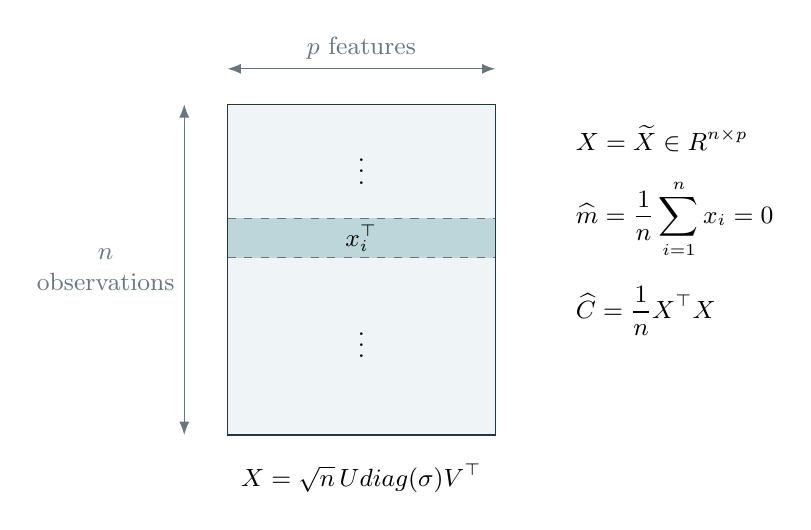
\begin{tikzpicture}[x=1cm,y=1cm]
\fill[accent!7] (0,0) rectangle(3.4,4.2);
\fill[accent!28] (0,2.25) rectangle(3.4,2.75);
\draw[ink] (0,0) rectangle(3.4,4.2);
\draw[guide] (0,2.25)--(3.4,2.25) (0,2.75)--(3.4,2.75);
\node at (1.7,2.5) {$x_i^\top$};
\node at (1.7,3.45) {$\vdots$};\node at (1.7,1.25) {$\vdots$};
\draw[<->,muted] (0,4.65)--(3.4,4.65) node[midway,above] {$p$ features};
\draw[<->,muted] (-.55,0)--(-.55,4.2) node[midway,left,align=center] {$n$\\observations};
\node[align=left,anchor=west] at (4.3,2.6) {$X=\widetilde X\in\mathbb R^{n\times p}$\\[9pt]$\displaystyle\widehat m=\frac1n\sum_{i=1}^n x_i=0$\\[9pt]$\displaystyle\widehat C=\frac1nX^\top X$};
\node at (1.7,-.55) {$X=\sqrt n\,U\operatorname{diag}(\sigma)V^\top$};
\end{tikzpicture}
\end{document}
